\documentclass{standalone}
\usepackage{tikz}
\usepackage{float}
\usepackage{amsmath}
\usepackage{lmodern}
\usepackage{amssymb}
\usetikzlibrary{calc}
\usetikzlibrary{hobby}
\usepackage{nicefrac}
\usetikzlibrary{decorations.markings}
\usetikzlibrary{patterns, patterns.meta}
\usetikzlibrary{shapes}
\usetikzlibrary{shapes.misc}
\usepackage{pgfplots}
\pgfplotsset{compat=1.18}
\begin{document}
\centering

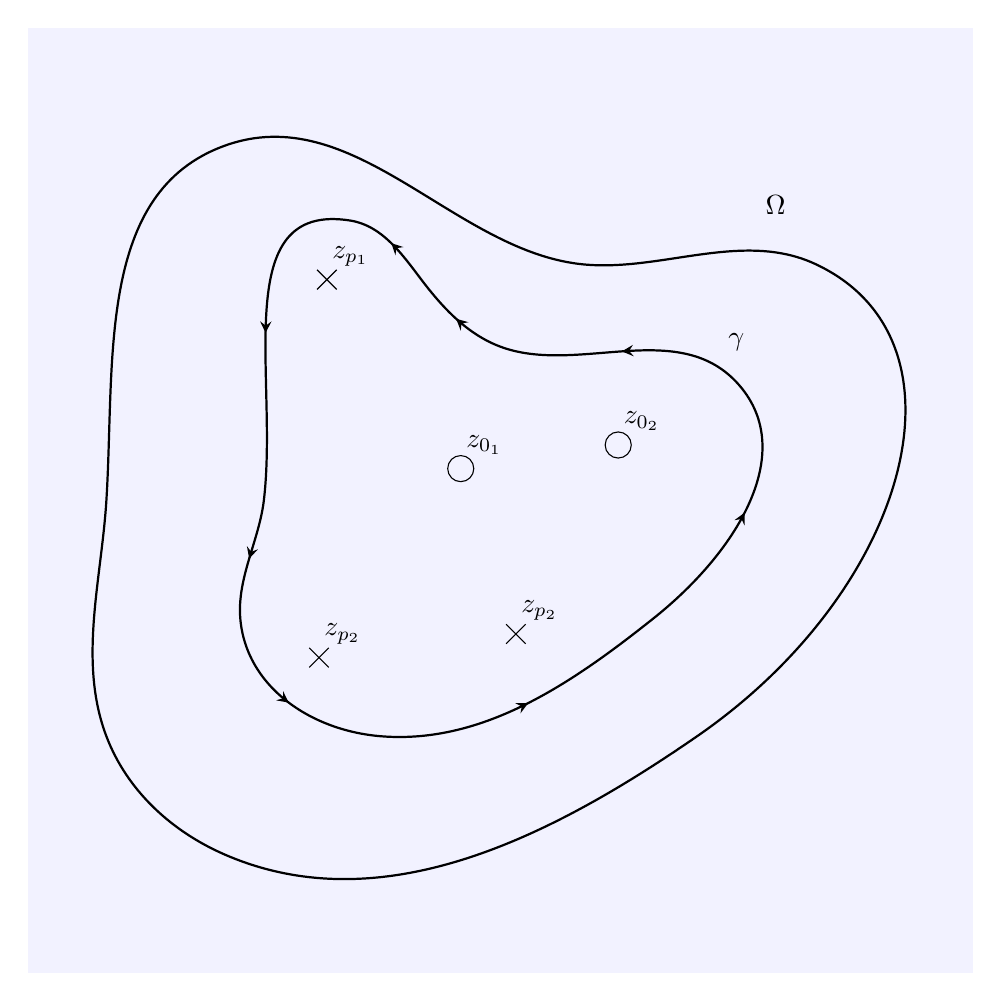
\begin{tikzpicture}
    \colorlet{BlueBackground}{blue!5}
    % Background for entire canvas
    \fill[BlueBackground] (-6,-6) rectangle (6,6);
    \tikzset{
      cross/.style={cross out, draw=red, fill=none, minimum size=2*(#1-\pgflinewidth), inner sep=0pt, outer sep=0pt,line width = 0.8pt}, cross/.default={2.8pt},
    % style to apply some styles to each segment of a path
    on each segment/.style={
      decorate,
      decoration={
        show path construction,
        moveto code={},
        lineto code={
          \path [#1]
          (\tikzinputsegmentfirst) -- (\tikzinputsegmentlast);
        },
        curveto code={
          \path [#1] (\tikzinputsegmentfirst)
          .. controls
          (\tikzinputsegmentsupporta) and (\tikzinputsegmentsupportb)
          ..
          (\tikzinputsegmentlast);
        },
        closepath code={
          \path [#1]
          (\tikzinputsegmentfirst) -- (\tikzinputsegmentlast);
        },
      },
    },
    % style to add an arrow in the middle of a path
    mid arrow/.style={postaction={decorate,decoration={
          markings,
          mark=at position .5 with {\arrow[#1]{stealth}}
        }}},
  }
    % draw omega space
    \path [draw=black,thick]
    (2.5,-3) to[closed, curve through =
    { (-3.5,-4.5) (-5,-3) (-5,0) (-3.5,4.5) (1,3) }] (4,3);
    \draw[color=black] (3.5,3.5) node[above] {$\Omega$};

    % draw contour around poles
    \path [draw=black,thick,postaction={on each segment={mid arrow=black}}]
    (3,1.5) to[closed, curve through =
    { (0,1.95) (-1,2.8) (-1.9,3.55) (-3,0) (-3.3,-1.5) (-1.5,-3) }] (1.95,-1.5);
    \node at (3,2) {\textcolor{black}{$\mathcal{\gamma}$}};

    % draw zeros
    \node[solid, circle,draw=black] at (-0.5,0.4) {};
    \node at (-0.2,0.7) {\textcolor{black}{$z_{0_1}$}};

    \node[solid, circle,draw=black] at (1.5,0.7) {};
    \node at (1.8,1.0) {\textcolor{black}{$z_{0_2}$}};
    
    %draw poles
    \node[solid, cross out,draw=black] at (-2.2,2.8) {};
    \node at (-1.9,3.1) {\textcolor{black}{$z_{p_1}$}};
    
    \node[solid, cross out,draw=black] at (-2.3,-2.0) {};
    \node at (-2.0,-1.7) {\textcolor{black}{$z_{p_2}$}};

    \node[solid, cross out,draw=black] at (0.2,-1.7) {};
    \node at (0.5,-1.4) {\textcolor{black}{$z_{p_2}$}};
    


\end{tikzpicture}

\end{document}
